\documentclass[a4pape, 11pt, english]{article}
\usepackage[margin=1in,footskip=0.25in]{geometry}
\usepackage{natbib}

%\usepackage{cite}
\usepackage{amsmath,amssymb,amsfonts}
\usepackage{algorithmic}
\usepackage{graphicx}
\usepackage{textcomp}
\usepackage{xcolor}

\usepackage[hyphens]{url} % To wrap urls on multiple lines: https://tex.stackexchange.com/questions/115690/urls-in-bibliography-latex-not-breaking-line-as-expected

\begin{document}
\title{Deep Reinforcement Learning Project}
\author{Thomas Fishwick}
\date{} % hide the date
\maketitle

\begin{abstract}
TODO: Abstract

Our code is available at this link \url{https://github.com/SL477/DRL-coursework}.
\end{abstract}

\section{Main problem: Starship Saboteur}
% describe the q-learning algorithm and my implementation of it
% describe some key parameters
\subsection{Define an environment and the problem to be solved}
%Here our agent will be teleported into a random free location on a spaceship (i.e. not blocked by any obstacles). Our agent will need to disable the spaceship's reactor by standing upon a certain location. Avoid the traps (which deal damage when stepped on) and navigate through the ship. Then go to the random beam-out location (which will also be an empty square) and escape before the max allowed turns, after that the ship will open the airlocks to immediately kill the agent.

%The agent will be able to 'see' the area around it not blocked by walls/other obstacles. Doors will count as obstacles to vision, but not to the agent. Its next objective's direction will be fed to it, along with its current health.

Our agent will start in a random empty location in the map shown in Figure \ref{fig:basic_map}. It has two positive reward points, the darker green point is the one with the highest reward and the lighter green point will terminate the training episode. The yellow points are negative reward points, they also deduct health points and if the agent's health drops to zero or less this will also terminate the episode. The agent can transition to any adjacent cell as long as it is not a wall. Currently the doors are only decorative items.

\textbf{The story version:}
Fired from a Solar Federation Space Force Infiltrator, our intrepid Space Marine Commando robot exits its boarding pod in a random place in the Custodian warship. Its mission is to cripple the ship's reactor before its crew are revived from stasis by planting a timed explosive on it. Its survival is optional, after it has completed its mission the robot can escape back to where a shuttle has cut a hole into the ship to retrieve it. But if the robot is destroyed, well we can always build more robots.
% harpoon line has been fired into the ship to retrieve it.

We will be using Q-learning to 'solve' this environment. Q-learning attempts to work out the cost/benefit of going from one state to the various other states around it based on their current and future rewards. Figure \ref{fig:basic_map_graph} shows which nodes are accessible to each other.

\begin{figure}[h!]
	\begin{center}
		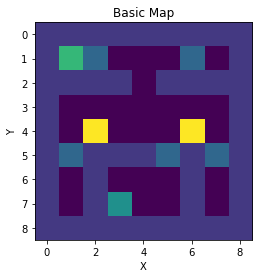
\includegraphics{img/basic_map.png}
		\caption{Green: reward points, yellow: obstacles, blue: doors, dark purple: empty space, light purple: walls}
		\label{fig:basic_map}
	\end{center}
\end{figure}

\begin{figure}[h!]
	\begin{center}
		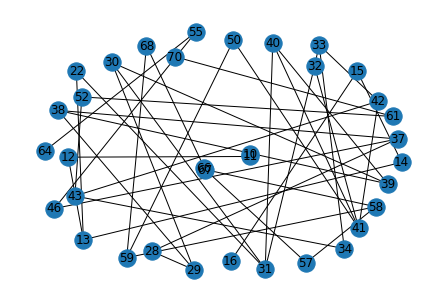
\includegraphics[scale=0.5]{img/basic_map_graph.png}
		\caption{Nodes with access to one another}
		\label{fig:basic_map_graph}
	\end{center}
\end{figure}


\subsection{Define a state transition function and the reward function}
To make our list of states we flatten the 2D map into an array. To flip from the array to the map we can get the row by integer dividing the index by the height of the map and the column by taking the modulus of the index by the width.

For the reward function we create a matrix with one state per row and one action per column. Using a lookup back to the map we get the code of the cell and lookup its reward (table \ref{tab:table1}). As the agent is only allowed to claim the primary objective once per episode the reward is set to zero once it has been claimed by the agent.

\begin{table}[h!]%[htbp]
	\begin{center}
		\caption{Rewards}
		\label{tab:table1}
		\begin{tabular}{|c|c|}
			\hline
			\textbf{Code} & \textbf{Reward} \\
			\hline
			Empty space & 0 \\
			\hline
			Wall & 0 \\
			\hline
			Door & 0 \\
			\hline
			The primary goal (the reactor control panel) & 50 \\
			\hline
			The secondary goal (the escape route) & 30 \\
			\hline
			A trap & -10 \\
			\hline
		\end{tabular}
	\end{center}
\end{table}



\subsection{Set up the Q-learning parameters (gamma, alpha) and policy}
For the Q-learning algorithm we have implemented it as a function (run\_q\_learning\_basic), with the parameters alpha, gamma, epsilon and num episodes.

Alpha, the learning rate, we have set as 1.

Gamma, the discount factor for future rewards, we set as 0.8.

Epsilon, the chance of choosing the policy 'exploit' over 'explore', we set as 0.9.

Num\_episodes, the number of learning episodes, we set as 1000.

\subsection{Run the Q-learning algorithm and represent its performance}
The Q-learning algorithm is:

$Q[s, a] = Q[s, a] + \alpha * R[s, a] + \gamma * (max(Q[s]) - Q[s, a])$

With the exploit/explore part given by:

if RandomNumber $> \epsilon$ then explore, otherwise exploit.

The algorithm takes 22.5 seconds to run on my PC. In Figure \ref{fig:firstparamsRewardVQVar} we can see the mean rewards versus their corresponding Q variances. The mean total health stayed at roughly 100, with at least one iteration within each iteration doing something to reduce its health. Most of the iteration's mean rewards were around 50, indicating that they were only going for one of the reward points (fortunately the higher reward point).

\begin{figure}[h!]
	\begin{center}
		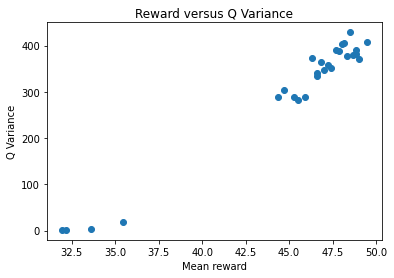
\includegraphics[scale=0.8]{img/firstparamsRewardVQVarWithEarlyStopping.png}
		\caption{Reward Versus Variance, for Alpha = 1, Gamma = 0.8, Epsilon = 0.9, for 27 rounds of 1000 iterations of training}
		\label{fig:firstparamsRewardVQVar}
	\end{center}
\end{figure}

It also looks like those which converged fastest were also the ones to get the lowest reward (around 30), they likely found that one first and did not explore enough to find the other reward point.

\subsection{Repeat the experiment with different parameter values, and policies}

\subsection{Analyse the results quantitatively and qualitatively}

\section{Implement DQN with two improvements}

\subsection{Analyse the results quantitatively and qualitatively}

\section{Apply the RL algorithm of your choice (from rllib) to one of the Atari Learning Environment. Briefly present the algorithm and justify your choice}

\subsection{Analyse the results quantitatively and qualitatively}

\section{Implementation of PPO or SAC}

\section{Summary of contribution}
100\% me

%\bibliographystyle{agsm} % using https://www.imperial.ac.uk/media/imperial-college/administration-and-support-services/library/public/LaTeX-example-Harvard-apr-2019.pdf to get Harvard style references
\bibliography{MyLibrary}
\end{document}